% file for pdflatex.exe

% process.tex v1.5.1 (c) | Copyright 2024 Daniel E. Janusch

% This file is licensed by https://raw.githubusercontent.com/drizzt536/files/main/LICENSE
% and may be copied ONLY IN ITS ENTIRETY under penalty of law.

\documentclass[12pt]{article}

\usepackage{amssymb, latexsym, amsmath, pgfplots, xcolor, hyperref, xurl}

\usepackage[margin=1in]{geometry}
\addtolength \topmargin {-0.5in}

\providecommand \floor [1]{\left\lfloor #1 \right\rfloor}
\providecommand \ceil [1]{ \left\lceil  #1 \right\rceil}
\providecommand \round [1]{\left\lfloor #1 \right\rceil}
\providecommand \trunc [1]{\left\lceil  #1 \right\rfloor}
\providecommand \pgrp [1]{\left( #1 \right)}   % paren group
\providecommand \bgrp [1]{\left[ #1 \right]}   % bracket group
\providecommand \cgrp [1]{\left\{ #1 \right\}} % curly (bracket) group.
\providecommand \abs [1]{\left| #1 \right|}
\providecommand \sgn {\mathrm{sgn}\,}
\providecommand \sgnf [1]{\mathrm{sgn}\!\pgrp{#1}}
\providecommand \dx {\df x}
\providecommand \dt {\df t}
\providecommand \df [1]{\mathrm d #1}
\providecommand \dstyle {\displaystyle}

\definecolor{lightgray}{RGB}{170, 170, 170}
\definecolor{dimblue}{RGB}{30, 30, 165}

\providecommand \darkMode 1
\ifnum \darkMode = 0
	% light mode
	\colorlet{bgcolor}{white}
	\colorlet{fgcolor}{black}

	\definecolor{dimred}{RGB}{165, 30, 30}
	\definecolor{dimgreen}{RGB}{30, 105, 30}
	\definecolor{gridgray}{RGB}{191, 191, 191}
\else
	\colorlet{bgcolor}{black}
	\colorlet{fgcolor}{lightgray}

	\definecolor{dimred}{RGB}{127, 0, 0}
	\definecolor{dimgreen}{RGB}{0, 71, 0}
	\definecolor{gridgray}{RGB}{60, 60, 60}
\fi

\color{fgcolor}
\pagecolor{bgcolor}

\pgfplotsset{
	compat = 1.18,
	width = 3in,
	points/.style n args = {1}{
		mark options = {
			draw = #1,
			fill = #1,
		},
		only marks,
		mark = *,
		line width = 0.6pt,
		mark size = 1.2pt,
		forget plot,
	},
	holes/.style n args = {1}{
		points = {#1},
		mark options = {
			draw = #1,
			fill = bgcolor,
		},
	}
}

\begin{document}

\phantomsection
\addcontentsline{toc}{section}{Title \& Introduction}
\phantomsection

\title{Integrating Functions with Countably-Many Jump Discontinuities}
\author{Daniel E. Janusch}
\date{September 5, 2024, 9:55pm MST}
\maketitle

	\indent While applications don't immediately come to attention, the pursuit of knowledge and
	mathematical literacy is enough in itself. Godfrey Harold Hardy (1940), a 20th-century
	mathematician famously said ``No discovery of mine has made, or is likely to make, directly
	or indirectly, for good or for ill, the least difference to~...~the world" (A Mathematician's
	Apology, 1st ed., p. 49); his work is now used everywhere in critical fields like
	cryptography.

	\indent For the following process to work, the functions are limited to a countable amount of
	jump discontinuities, since if there is an uncountable amount, then by definition, the
	discontinuities can't be listed out, and step~2 won't work. It makes it much easier to assume
	that there are no discontinuities other than the jump discontinuities, but the main essence of
	the steps should be about the same in that case. This process pertains to step functions like
	$\floor x$ (floor) and $\ceil x$ (ceiling). The notation used will be as follows: $f(x)$ is
	the full function with the step functions in it and  $g(x)$ is the same function but with the
	step functions removed. For instance, if $f(x)$ is any of $x^2$, $\floor{x}^2$, $\floor{x^2}$,
	or $x\floor x$, then $g(x) = x^2$. Functions like $f(x) = \floor{x}^2 - 2\floor x$ are
	continuous analogs of discrete functions (you could replace $\floor x$ with $n$ and have no
	$x$s left over), so this process could introduce a way of integrating discrete functions.

\phantomsection
\addcontentsline{toc}{section}{Step 1: Define a Function to Integrate}
\phantomsection
\section*{Step 1: Define a Function to Integrate}

	\indent\indent You can use almost any function you want, but if it is too general steps 3 or 4
	might not work. Some possible examples for $f(x)$ are $\floor x$, $\floor{\sin\pi x}$,
	$\floor{x^2 - x + 1}$, or $\floor{\frac 1x}$. Usually, if you have anything in terms of the
	ceiling, rounding, or truncating functions, you will want to convert them to the floor
	function with these formulas: $\mathrm{round}(x) = \floor{x + \frac12}$, $\ceil x = -
	\floor{-x}$, and $\mathrm{truncate}(x) = \floor{\abs x}\sgn x$. Sometimes you will need to pay
	attention to the integral boundaries, as for most functions they can be 0 and $x$, but, for
	example, for $f(x) = \floor{\frac 1x}$, they should be 1 and $x$. The lower bound should be
	wherever the integral is zero. Don't use a na{\"\i}ve approach like $\int\floor x\!\dx=x\!
	\floor x+c$; while taking the derivative of both sides technically does give the same
	function, it is not correct because it is missing $-\frac12\!\floor x\!(\floor x + 1)$. This
	is because $\dstyle\lim_{x\to a}\frac{\df{\floor x}}\dx(a) = 0$ for any constant $a$, so
	$\floor x$ can just be treated as a constant when taking derivatives. Here are a couple
	example graphs.

	\begin{figure}[ht]
		\centering
		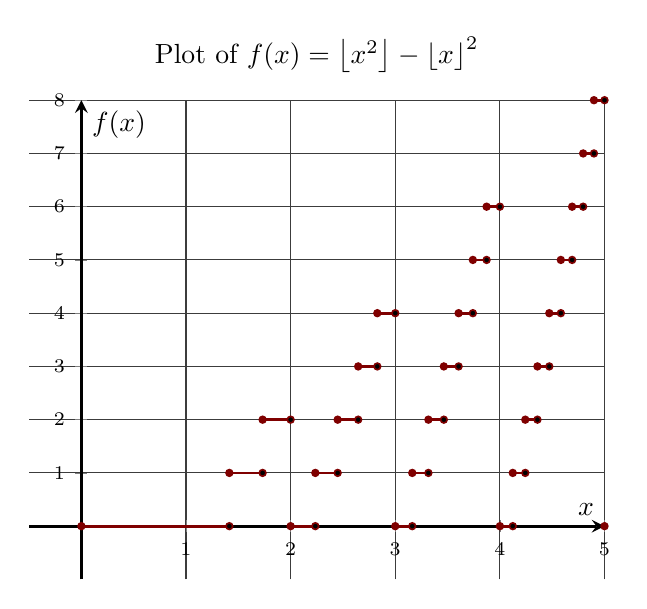
\begin{tikzpicture}
			\begin{axis}[
				clip = false,
				width = 3.5in,
				xmin=-0.5, xmax=5, xtick={1,2,3,4,5}, xlabel=$x$,
				ymin=-1  , ymax=8, ytick={1,...,8  }, ylabel=$f(x)$,
				tick label style={font=\scriptsize},
				% extra x ticks = {sqrt(2), sqrt(6), sqrt(12), sqrt(20)},
				% extra x tick labels = {$\sqrt 2$, $\sqrt 6$, $\sqrt{12}$, $\sqrt{20}$},
				axis lines = middle,
				grid = both,
				grid style = {draw = gridgray},
				line width = 1.01pt,
				title = {Plot of $f(x) = \floor{x^2} - \floor x^2$},
			]

				\addplot[color=dimred, domain=sqrt( 0):sqrt( 2), samples=2]{0};
				\addplot[color=dimred, domain=sqrt( 2):sqrt( 3), samples=2]{1};
				\addplot[color=dimred, domain=sqrt( 3):sqrt( 4), samples=2]{2};
				\addplot[color=dimred, domain=sqrt( 4):sqrt( 5), samples=2]{0};
				\addplot[color=dimred, domain=sqrt( 5):sqrt( 6), samples=2]{1};
				\addplot[color=dimred, domain=sqrt( 6):sqrt( 7), samples=2]{2};
				\addplot[color=dimred, domain=sqrt( 7):sqrt( 8), samples=2]{3};
				\addplot[color=dimred, domain=sqrt( 8):sqrt( 9), samples=2]{4};
				\addplot[color=dimred, domain=sqrt( 9):sqrt(10), samples=2]{0};
				\addplot[color=dimred, domain=sqrt(10):sqrt(11), samples=2]{1};
				\addplot[color=dimred, domain=sqrt(11):sqrt(12), samples=2]{2};
				\addplot[color=dimred, domain=sqrt(12):sqrt(13), samples=2]{3};
				\addplot[color=dimred, domain=sqrt(13):sqrt(14), samples=2]{4};
				\addplot[color=dimred, domain=sqrt(14):sqrt(15), samples=2]{5};
				\addplot[color=dimred, domain=sqrt(15):sqrt(16), samples=2]{6};
				\addplot[color=dimred, domain=sqrt(16):sqrt(17), samples=2]{0};
				\addplot[color=dimred, domain=sqrt(17):sqrt(18), samples=2]{1};
				\addplot[color=dimred, domain=sqrt(18):sqrt(19), samples=2]{2};
				\addplot[color=dimred, domain=sqrt(19):sqrt(20), samples=2]{3};
				\addplot[color=dimred, domain=sqrt(20):sqrt(21), samples=2]{4};
				\addplot[color=dimred, domain=sqrt(21):sqrt(22), samples=2]{5};
				\addplot[color=dimred, domain=sqrt(22):sqrt(23), samples=2]{6};
				\addplot[color=dimred, domain=sqrt(23):sqrt(24), samples=2]{7};
				\addplot[color=dimred, domain=sqrt(24):sqrt(25), samples=2]{8};

				\addplot[points=dimred] coordinates {
					(0, 0)
					(sqrt( 2), 1) (sqrt( 3), 2)
					(sqrt( 4), 0) (sqrt( 5), 1)
					(sqrt( 6), 2) (sqrt( 7), 3)
					(sqrt( 8), 4) (sqrt( 9), 0)
					(sqrt(10), 1) (sqrt(11), 2)
					(sqrt(12), 3) (sqrt(13), 4)
					(sqrt(14), 5) (sqrt(15), 6)
					(sqrt(16), 0) (sqrt(17), 1)
					(sqrt(18), 2) (sqrt(19), 3)
					(sqrt(20), 4) (sqrt(21), 5)
					(sqrt(22), 6) (sqrt(23), 7)
					(sqrt(24), 8) (sqrt(25), 0)
				};

				\addplot[holes=dimred] coordinates {
					(sqrt( 2), 0) (sqrt( 3), 1)
					(sqrt( 4), 2) (sqrt( 5), 0)
					(sqrt( 6), 1) (sqrt( 7), 2)
					(sqrt( 8), 3) (sqrt( 9), 4)
					(sqrt(10), 0) (sqrt(11), 1)
					(sqrt(12), 2) (sqrt(13), 3)
					(sqrt(14), 4) (sqrt(15), 5)
					(sqrt(16), 6) (sqrt(17), 0)
					(sqrt(18), 1) (sqrt(19), 2)
					(sqrt(20), 3) (sqrt(21), 4)
					(sqrt(22), 5) (sqrt(23), 6)
					(sqrt(24), 7) (sqrt(25), 8)
				};
			\end{axis}
		\end{tikzpicture}
		\hfill
		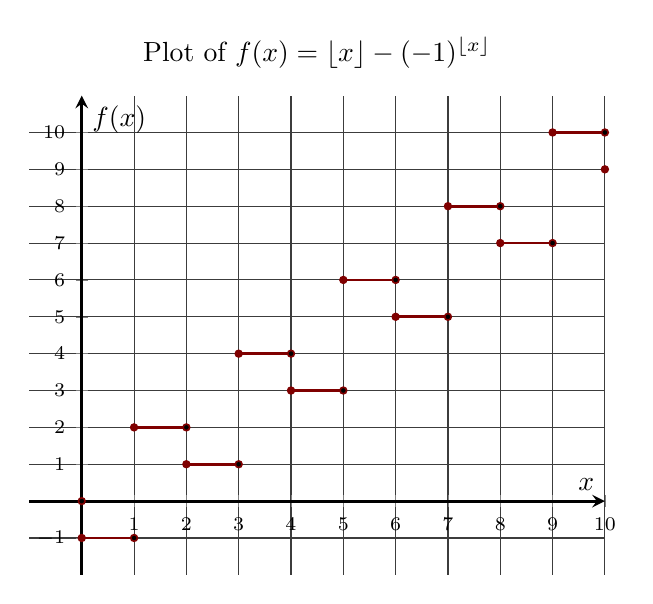
\begin{tikzpicture}
			\begin{axis}[
				clip = false,
				width = 3.5in,
				xmin=-1, xmax=10, xtick={ 1,...,10}, xlabel = $x$,
				ymin=-2, ymax=10, ytick={-1,...,10}, ylabel = $f(x)$,
				tick label style={font=\scriptsize},
				line width = 1.01pt,
				axis lines = center,
				samples = 10,
				ymin = -2,
				ytick distance = 2,
				ymax = 11,
				grid = both,
				grid style = {draw = gridgray},
				title = {Plot of $f(x) = \floor x - (-1)^{\floor x}$},
			]

				\addplot[color=dimred, domain=0:1 , samples=2]{-1};
				\addplot[color=dimred, domain=1:2 , samples=2]{2};
				\addplot[color=dimred, domain=2:3 , samples=2]{1};
				\addplot[color=dimred, domain=3:4 , samples=2]{4};
				\addplot[color=dimred, domain=4:5 , samples=2]{3};
				\addplot[color=dimred, domain=5:6 , samples=2]{6};
				\addplot[color=dimred, domain=6:7 , samples=2]{5};
				\addplot[color=dimred, domain=7:8 , samples=2]{8};
				\addplot[color=dimred, domain=8:9 , samples=2]{7};
				\addplot[color=dimred, domain=9:10, samples=2]{10};

				\addplot[holes=dimred] coordinates {
					(0, 0) (1, -1)
					(2, 2) (3, 1)
					(4, 4) (5, 3)
					(6, 6) (7, 5)
					(8, 8) (9, 7)
					(10, 10)
				};

				\addplot[points=dimred] coordinates {
					(0, -1) (1, 2)
					(2, 1) (3, 4)
					(4, 3) (5, 6)
					(6, 5) (7, 8)
					(8, 7) (9, 10)
					(10, 9)
				};
			\end{axis}
		\end{tikzpicture}
	\end{figure}

\phantomsection
\addcontentsline{toc}{section}{Step 2: Split at the Jumps and Integrate Separately}
\phantomsection
\section*{Step 2: Split at the Jumps and Integrate Separately}

	\indent\indent Since $f(x)$ is not continuous, you need to figure out where the value of
	$f(x)$ changes, or where the $n$th jump discontinuity is. Then you split the integral by these
	boundaries and integrate each interval individually. Sometimes this can be slightly trickier
	if you have something like $f(x)=\sqrt{\floor x}$ because not all the output values are at
	integers. You will benefit from using a different strategy for periodic functions like
	$\floor{\cos x}$ to take advantage of their periodicity. Splitting at jumps is a similar
	method to how you integrate piecewise functions, although in piecewise functions you split the
	integral at the piece boundaries instead of just at jumps (Calculus, Larson \& Edwards, 2010).

	\phantomsection
	\addcontentsline{toc}{subsection}{Example 1}
	\phantomsection
	\subsection*{Example 1}

		\begin{minipage}{0.5\textwidth}
			\begin{align*}
				f(x)                                    := & \, \floor{\frac x2}\\
				g(x)                                     = & \, \frac x2\\
				g^{-1}(x)                                = & \, 2x\\
				\int_{2n}^{2(n+1)}\hspace{-1.3em}f(t)\dt = & \int_{2n}^{2n+2}
														\floor{\frac t2}\!\dt
			\end{align*}
		\end{minipage}
		\begin{minipage}{0.5\textwidth}
			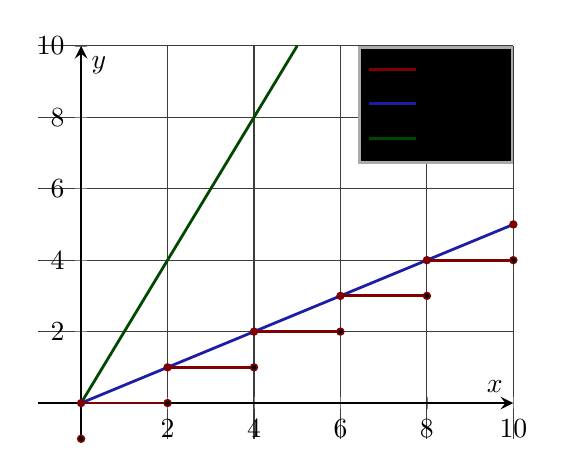
\begin{tikzpicture}
				\begin{axis}[
					clip = false,
					xlabel = $x$,
					ylabel = $y$,
					axis lines = middle,
					xmin = -1, xmax = 10,
					ymin = -1, ymax = 10,
					xtick = {2, 4, 6, 8, 10},
					ytick = {2, 4, 6, 8, 10},
					grid = both,
					grid style = {draw = gridgray},
					line width = 1.01pt,
					legend cell align = left,
					legend style = {
						font = \small,
						fill = bgcolor,
						draw = fgcolor,
						at = {(1, 1)},
						anchor = north east
					},
				]

					\addplot[color=dimblue, domain=0:10, samples=2, forget plot]{x/2};
					\addplot[color=dimgreen, domain=0:5, samples=2, forget plot]{2*x};

					\addplot[color=dimred, domain=0:2, samples=2, forget plot]{0};
					\addplot[color=dimred, domain=2:4, samples=2, forget plot]{1};
					\addplot[color=dimred, domain=4:6, samples=2, forget plot]{2};
					\addplot[color=dimred, domain=6:8, samples=2, forget plot]{3};
					\addplot[color=dimred, domain=8:10, samples=2, forget plot]{4};

					\addplot[points=dimred] coordinates {
						(0, 0) (2, 1)
						(4, 2) (6, 3)
						(8, 4) (10, 5)
					};

					\addplot[holes=dimred] coordinates {
						(0, -1) (2, 0)
						(4, 1) (6, 2)
						(8, 3) (10, 4)
					};

					\addlegendimage{dimred, line legend}
					\addlegendentry{$f(x)$}
					\addlegendimage{dimblue, line legend}
					\addlegendentry{$g(x)$}
					\addlegendimage{dimgreen, line legend}
					\addlegendentry{$g^{-1}(x)$}
				\end{axis}
			\end{tikzpicture}
		\end{minipage}
		\vspace{0.2em}

		$f(x)$ on this interval will be the same value, so this is just the area of a rectangle.
		Ignore the discontinuities at the endpoints; they don't change the outcome of the
		integral.

		\begin{align*}
			\int_{2n}^{2n+2}\floor{\frac t2}\!\dt
			= \floor{\frac{2n}2} (2n+2-2n)
			= \floor n \cdot 2 = 2n
		\end{align*}

	\phantomsection
	\addcontentsline{toc}{subsection}{Example 2}
	\phantomsection
	\subsection*{Example 2}

		\begin{minipage}{0.5\textwidth}
			\begin{align*}
				f(x)     := & \, \big\lfloor x^2\big\rfloor\\
				g(x)      = & \, \phantom{\big\lfloor} x^2\\
				g^{-1}(x) = & \, \sqrt x\\
			\end{align*}
		\end{minipage}
		\begin{minipage}{0.5\textwidth}
			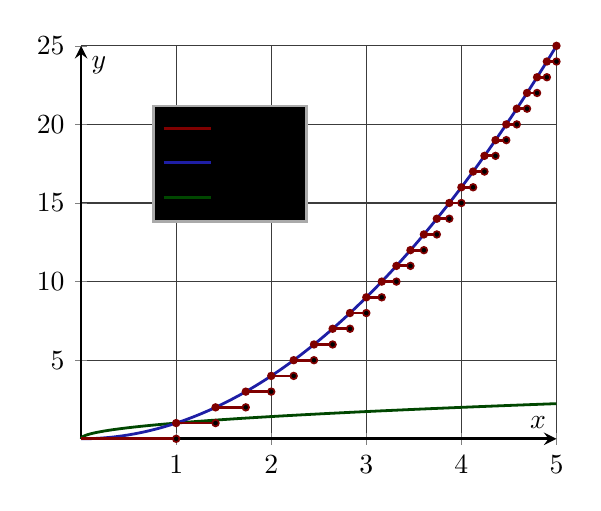
\begin{tikzpicture}
				\begin{axis}[
					clip = false,
					xlabel = $x$,
					ylabel = $y$,
					axis lines = middle,
					grid = both,
					grid style = {draw = gridgray},
					line width = 1.01pt,
					legend cell align = left,
					legend style = {
						font = \small,
						fill = bgcolor,
						draw = fgcolor,
						anchor = west,
						at = {(0.15, 0.7)},
					},
				]

					\addplot[color=dimgreen, samples=1000, domain=0:5, forget plot]{sqrt(x)};
					\addplot[color=dimblue, samples=1000, domain=0:5, forget plot]{x^2};

					\addplot[color=dimred, domain=0.000:1.000, samples=3, forget plot]{0};
					\addplot[color=dimred, domain=1.000:1.414, samples=3, forget plot]{1};
					\addplot[color=dimred, domain=1.415:1.732, samples=3, forget plot]{2};
					\addplot[color=dimred, domain=1.733:2.000, samples=3, forget plot]{3};
					\addplot[color=dimred, domain=2.000:2.236, samples=3, forget plot]{4};
					\addplot[color=dimred, domain=2.237:2.449, samples=3, forget plot]{5};
					\addplot[color=dimred, domain=2.450:2.645, samples=3, forget plot]{6};
					\addplot[color=dimred, domain=2.646:2.828, samples=3, forget plot]{7};
					\addplot[color=dimred, domain=2.829:3.000, samples=3, forget plot]{8};
					\addplot[color=dimred, domain=3.000:3.162, samples=3, forget plot]{9};
					\addplot[color=dimred, domain=3.163:3.316, samples=3, forget plot]{10};
					\addplot[color=dimred, domain=3.317:3.464, samples=3, forget plot]{11};
					\addplot[color=dimred, domain=3.465:3.605, samples=3, forget plot]{12};
					\addplot[color=dimred, domain=3.606:3.741, samples=3, forget plot]{13};
					\addplot[color=dimred, domain=3.742:3.872, samples=3, forget plot]{14};
					\addplot[color=dimred, domain=3.873:4.000, samples=3, forget plot]{15};
					\addplot[color=dimred, domain=4.000:4.123, samples=3, forget plot]{16};
					\addplot[color=dimred, domain=4.124:4.242, samples=3, forget plot]{17};
					\addplot[color=dimred, domain=4.245:4.358, samples=3, forget plot]{18};
					\addplot[color=dimred, domain=4.359:4.472, samples=3, forget plot]{19};
					\addplot[color=dimred, domain=4.473:4.582, samples=3, forget plot]{20};
					\addplot[color=dimred, domain=4.583:4.690, samples=3, forget plot]{21};
					\addplot[color=dimred, domain=4.691:4.795, samples=3, forget plot]{22};
					\addplot[color=dimred, domain=4.796:4.898, samples=3, forget plot]{23};
					\addplot[color=dimred, domain=4.899:5.001, samples=3, forget plot]{24};

					\addplot[points=dimred] coordinates {
						(1, 1)
						(sqrt(2), 2) (sqrt(3), 3)
						(sqrt(4), 4) (sqrt(5), 5)
						(sqrt(6), 6) (sqrt(7), 7)
						(sqrt(8), 8) (sqrt(9), 9)
						(sqrt(10), 10) (sqrt(11), 11)
						(sqrt(12), 12) (sqrt(13), 13)
						(sqrt(14), 14) (sqrt(15), 15)
						(sqrt(16), 16) (sqrt(17), 17)
						(sqrt(18), 18) (sqrt(19), 19)
						(sqrt(20), 20) (sqrt(21), 21)
						(sqrt(22), 22) (sqrt(23), 23)
						(sqrt(24), 24) (sqrt(25), 25)
					};

					\addplot[holes=dimred] coordinates {
						(1, 0)
						(sqrt(2), 1) (sqrt(3), 2)
						(sqrt(4), 3) (sqrt(5), 4)
						(sqrt(6), 5) (sqrt(7), 6)
						(sqrt(8), 7) (sqrt(9), 8)
						(sqrt(10), 9) (sqrt(11), 10)
						(sqrt(12), 11) (sqrt(13), 12)
						(sqrt(14), 13) (sqrt(15), 14)
						(sqrt(16), 15) (sqrt(17), 16)
						(sqrt(18), 17) (sqrt(19), 18)
						(sqrt(20), 19) (sqrt(21), 20)
						(sqrt(22), 21) (sqrt(23), 22)
						(sqrt(24), 23) (5, 24)
					};

					\addlegendimage{dimred, line legend} \addlegendentry{$f(x)$}
					\addlegendimage{dimblue, line legend} \addlegendentry{$g(x)$}
					\addlegendimage{dimgreen, line legend} \addlegendentry{$g^{-1}(x)$}
				\end{axis}
			\end{tikzpicture}
		\end{minipage}

		doing the same thing as in example 1, we get:

		\begin{align*}
			\int_{\sqrt n}^{\sqrt{n+1}}f(t)\dt = f(\sqrt n)\pgrp{\sqrt{n+1}-\sqrt n}
			= \floor x\sqrt{1+2x-2\sqrt{x^2+x}}\\
			\text{and in general, }\int_{g^{-1}(n)}^{g^{-1}(n+1)}f(t)\dt
			=f\pgrp{g^{-1}(n)}\bgrp{g^{-1}(n+1)-g^{-1}(n)}
		\end{align*}

		This general formula only works if $f(x)$ is constant in between discontinuities.
		Make sure you use the correct area formula for your function. For instance, If you
		have $f(x)=x\floor x$ then use the trapezoid area formula instead.

\phantomsection
\addcontentsline{toc}{section}{Step 3: Find the Sum of Each Partial Integral}
\phantomsection
\section*{Step 3: Find the Sum of Each Partial Integral}

	\indent\indent After you've figured out the closed form of the integral on each interval, you
	can use the additive interval property of integrals, where ``if $f$ is integrable on the three
	closed intervals determined by $a$, $b$, and $c$, then $\dstyle \int_a^b\!\!f(x)\dx=
	\int_a^c\!\!f(x)\dx+\int_c^b\!\!f(x)\dx$" (Calculus, Larson \& Edwards, 2010, p.
	276). Sum up the separate integrals and get the closed form on the whole interval. The
	following summation is impossible for a general $f(x)$, so you need to have a specific
	function for this step.

	\begin{align*}
		\int_{g^{-1}(0)}^{g^{-1}(k)}f(t)\dt=\sum_{j=1}^{k-1}\int_{g^{-1}(j)}^{g^{-1}(j+1)}
			f(t)\dt
	\end{align*}

	\indent Oftentimes you can end up with something complicated as the closed form, like the
	general harmonic sequence, or a difference of Hurwitz Zeta functions. Other times the sum
	can just be impossible to get a closed form for.

	\phantomsection
	\addcontentsline{toc}{subsection}{Example}
	\phantomsection
	\subsection*{Example}

		\begin{minipage}{0.5\textwidth}
			\begin{align*}
				f(x)     := & \, \floor x\\
				g(x)      = & \, \phantom\lfloor x\\
				g^{-1}(x) = & \, \phantom\lfloor x
			\end{align*}
		\end{minipage}
		\begin{minipage}{0.5\textwidth}
			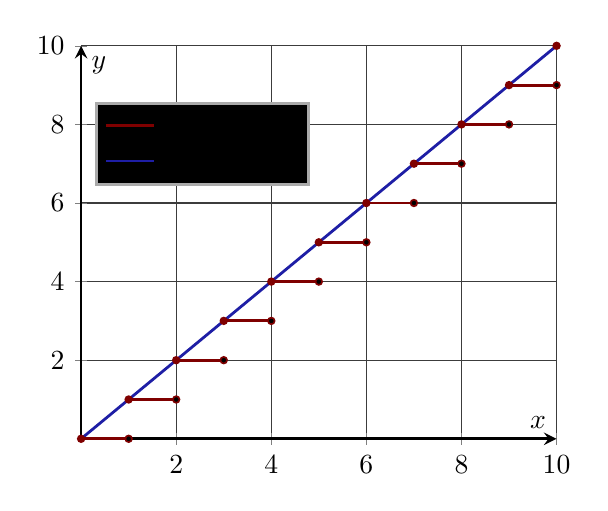
\begin{tikzpicture}
				\begin{axis}[
					clip = false,
					xlabel = $x$,
					ylabel = $y$,
					grid = both,
					grid style = {draw = gridgray},
					axis lines = center,
					line width = 1.01pt,
					legend cell align = left,
					legend style = {
						font = \small,
						fill = bgcolor,
						draw = fgcolor,
						anchor = west,
						at = {(0.03, 0.75)},
					},
				]

					\addplot[color=dimblue, domain=0:10, samples=2, forget plot]{x};

					\addplot[color=dimred, domain=0:1, forget plot]{0};
					\addplot[color=dimred, domain=1:2, forget plot]{1};
					\addplot[color=dimred, domain=2:3, forget plot]{2};
					\addplot[color=dimred, domain=3:4, forget plot]{3};
					\addplot[color=dimred, domain=4:5, forget plot]{4};
					\addplot[color=dimred, domain=5:6, forget plot]{5};
					\addplot[color=dimred, domain=6:7, forget plot]{6};
					\addplot[color=dimred, domain=7:8, forget plot]{7};
					\addplot[color=dimred, domain=8:9, forget plot]{8};
					\addplot[color=dimred, domain=9:10, forget plot]{9};

					\addplot[points=dimred] coordinates {
						(0, 0) (1, 1)
						(2, 2) (3, 3)
						(4, 4) (5, 5)
						(6, 6) (7, 7)
						(8, 8) (9, 9)
						(10, 10)
					};

					\addplot[holes=dimred] coordinates {
						(1, 0) (2, 1)
						(3, 2) (4, 3)
						(5, 4) (6, 5)
						(7, 6) (8, 7)
						(9, 8) (10, 9)
					};


					\addlegendimage{dimred, line legend}
					\addlegendentry{$f(x)$}
					\addlegendimage{dimblue, line legend}
					\addlegendentry{$g(x), g^{-1}(x)$}

				\end{axis}
			\end{tikzpicture}
		\end{minipage}

		\begin{align*}
			\int_0^k\floor t\dt
			= \sum_{j=0}^{k-1}\int_j^{j+1}\!\floor t\dt
			= \sum_{j=1}^{k-1}j\cdot(j+1-j)
			= \frac{k^2-k}2
		\end{align*}

\phantomsection
\addcontentsline{toc}{section}{Step 4: Integrate up to x}
\phantomsection
\section*{Step 4: Integrate up to $x$}

	\indent\indent To integrate up to $x$, you can once again use the additive interval property
	of integrals. The first integral (on the right) is from step~3, and the second is similar to
	in step~2. $g^{-1}(f(x))$ is the greatest $x$-value less than $x$ with a jump discontinuity.
	The formula for the second integral is not always correct; use the correct area formula for
	the section. It is the same process as in step~2 but using a subset of the interval.

	\begin{align*}
		\int_{g^{-1}(0)}^xf(t)   \dt & = \int_{g^{-1}(0)}^{g^{-1}(f(x))}f(t)\dt+\int_{g^{-1}
										(f(x))}^xf(t)\dt\\
		\int_{g^{-1}(f(x))}^xf(t)\dt & = f(x)\!\bgrp{x-g^{-1}(f(x))}
	\end{align*}

	\phantomsection
	\addcontentsline{toc}{subsection}{Example}
	\phantomsection
	\subsection*{Example}

		\begin{minipage}{0.5\textwidth}
			\begin{align*}
				f(x)     := & \, \floor x\\
				g(x)      = & \, \phantom\lfloor x\\
				g^{-1}(x) = & \, \phantom\lfloor x
			\end{align*}
		\end{minipage}
		\begin{minipage}{0.5\textwidth}
			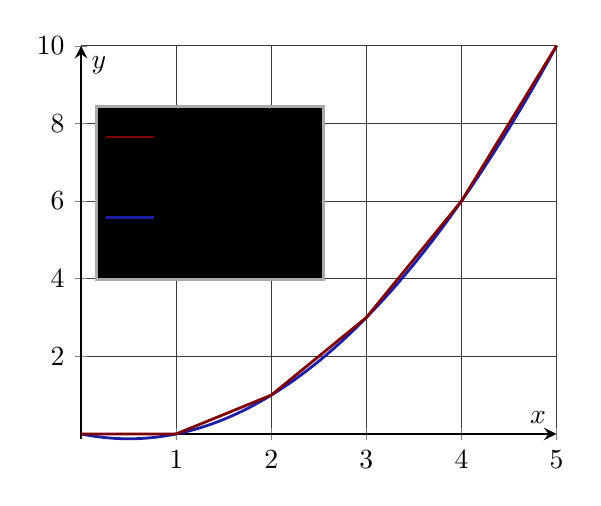
\begin{tikzpicture}
				\begin{axis}[
					clip = false,
					xlabel = $x$,
					ylabel = $y$,
					axis lines = center,
					samples = 2000,
					grid = both,
					grid style = {draw = gridgray},
					domain = 0:5,
					line width = 1.01pt,
					legend cell align = left,
					legend style = {
						font = \small,
						anchor = west,
						fill = bgcolor,
						draw = fgcolor,
						at = {(0.03, 0.625)},
					},
				]

					\addplot[color=dimblue, forget plot]{(x^2 - x) / 2};
					\addplot[color=dimred, forget plot]{
						(floor(x)^2 - floor(x)) / 2 + (x - floor(x)) * floor(x)
					};


					\addlegendimage{dimred, line legend}
					\addlegendentry{$\dstyle\int_0^x\floor t\dt$}

					\addlegendimage{empty legend} \addlegendentry[]{}
					\addlegendimage{empty legend} \addlegendentry[]{}

					\addlegendimage{dimblue, line legend}
					\addlegendentry{$\dstyle\int_0^x\!\bgrp{t-\frac12}\!\dt$}

					\addlegendimage{empty legend} \addlegendentry[]{}
					\addlegendimage{empty legend} \addlegendentry[]{}
				\end{axis}
			\end{tikzpicture}
		\end{minipage}

		\begin{align*}
			\int_{g^{-1}(0)}^x\hspace{-1.4em}f(t)\dt
			= \int_0^{\floor x}\hspace{-0.9em}\floor t\!\dt+\int_{\floor x}^x\hspace{-0.6em}
				\floor t\!\dt
			= \frac{\floor x^2-\floor x}2+(x-\floor x)\floor x
		\end{align*}

		Once you have this, you have found the principle indefinite integral. Add the constant of
		integration for the general answer.

\phantomsection
\addcontentsline{toc}{section}{Table of Results}
\phantomsection
\section*{Table of Results}

	\indent\indent Assume the bounds are $0$ and $x$ unless explicitly mentioned.

	\begin{minipage}{\textwidth}
		\centering
		\begin{align}
			& \int \! x \bmod c\; \dx = \dfrac{c^2}2\!\pgrp{\floor{\dfrac xc}+
										\dfrac xc\;\mathrm{mod}^2\,1}\\
			& \int \floor x\!\dx = \dfrac12\floor x(2x-\floor x-1)\\
			& \int \ceil  x\!\dx = \dfrac12\ceil x(2x-\ceil x+1)\\
			& \int \round x\!\dx = \dfrac12(\round x-1)(2x-\round x-1)\ni\round x=
								\mathrm{round}(x)\\
			& \int \trunc x\!\dx = \dfrac12\floor x(2x - \floor x - 1) + \min(0,x) \ni\trunc x =
								\mathrm{truncate}(x)\\
			& \int_1^x \!\!\!\floor{\log_b t}\!\dt = x \!\floor{\log_b t} + \dfrac b{b-1}\!
												\bgrp{1 - b^{\floor{\log_b t}}} \\
			& \int \!f \dx = \bgrp{x+\dfrac b{2a}}\!f-\dfrac{\abs bn}{2a}+\dfrac{\zeta\!\pgrp{-
							\dfrac12,\dfrac{b^2}{4a}+1+f-n}-\zeta\!\pgrp{-\dfrac12,\dfrac{b^2}{4a}
							+1}}{\sqrt a}\\
			& \ni f = \floor{ax^2 + bx + n} \notag
		\end{align}
	\end{minipage}

\phantomsection
\addcontentsline{toc}{section}{References}
\phantomsection
\section*{References}
	% I think these are in APA, but I don't really care.

	\begin{itemize}
		\item Hardy, G. H. (1940). A Mathematician's Apology (1st ed.). University of Alberta
			Mathematical Sciences Society.\\
			\url{https://www.arvindguptatoys.com/arvindgupta/mathsapology-hardy.pdf}\\

		\item Larson, R., \& Edwards, B. H. (2010). Calculus (9th ed.). Cengage Learning.\\
			\url{http://teacherpress.ocps.net/cynthiaandrews/files/2013/06/
			Calculus-9th-Edition-by-Ron-Larson-Bruce-H.-Edwards.pdf}
	\end{itemize}
	\vfill
	This document is licensed under
	\url{https://raw.githubusercontent.com/drizzt536/files/main/LICENSE}
	and may be copied ONLY IN ITS ENTIRETY under penalty of law.
	\vspace{0.5em}

\end{document}
